\documentclass[../piano-di-progetto.tex]{subfiles}

\begin{document}

  \subsection{Analisi}

  \subsubsection{Prospetto orario}
  Nel periodo di Analisi, la distribuzione oraria è la seguente:
  \begin{table}[H]
    \centering
    \begin{tabular}{lccccccc}
      Nominativo                & Re         & Am         & An         & Pt         & Pr         & Ve         & Ore totali \\
      Sofia Bononi              & -          & 8          & 14          & -          & -          & 9          & 31          \\
      Enrico Buratto            & -          & 14         & 8          & -          & -          & 8          & 30          \\
      Ian Nicolas Di Menna      & 9          & -          & 9          & -          & -          & 12          & 30          \\
      Alessandro Franchin       & 9          & -          & 9          & -          & -          & 13          & 31         \\
      Enrico Galdeman           & -          & 7          & 14          & -          & -          & 10          & 31          \\
      Nicholas Miazzo           & 10         & -          & 10          & -          & -          & 10         & 30         \\
      Marco Nardelotto          & -          & 9          & 9         & -          & -          & 13          & 31          \\
      \textbf{Ore totali ruolo} & \textbf{28} & \textbf{38} & \textbf{73} & \textbf{-} & \textbf{-} & \textbf{75} & \textbf{214}
    \end{tabular}
    \caption{Distribuzione oraria del periodo di Analisi}
  \end{table}


  Per facilitare la lettura della distribuzione oraria, i dati vengono rappresentati graficamente il seguente istogramma:
  \begin{figure}[H]
    \centering
    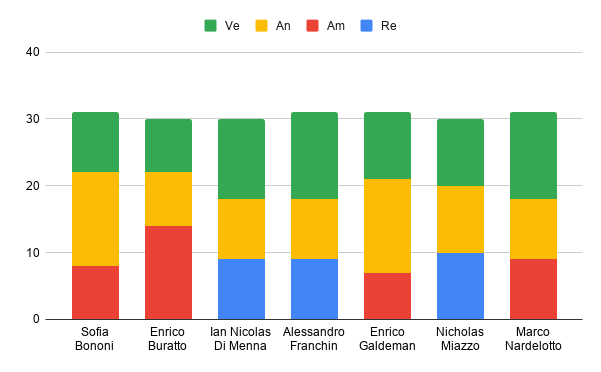
\includegraphics[width=12cm]{img/ore-analisi.png}
    \caption{Istogramma della distribuzione oraria del periodo di Analisi}
    \label{fig:ore-componente-analisi}
  \end{figure}

  \subsubsection{Prospetto economico}
  In questo del periodo, la suddivisione oraria e i costi per ruolo è la seguente:

  \begin{table}[H]
    \centering
    \begin{tabular}{lcc}
      Ruolo           & Ore previste & Costo      \\
      Responsabile    & 28           & € 840,00          \\
      Amministratore  & 38            & € 760          \\
      Analista        & 73            & -          \\
      Progettista     & -            & -          \\
      Programmatore   & 75            & -          \\
      Verificatore    & -            & € 1.125,00          \\
      \textbf{Totale} & \textbf{214}   & \textbf{€ 4.550,00}
    \end{tabular}
    \caption{Prospetto economico del periodo di Analisi}
  \end{table}


  Per facilitare la lettura della suddivisione oraria per ruolo, i dati vengono rappresentati graficamente mediante il seguente areogramma:
  \begin{figure}[H]
    \centering
    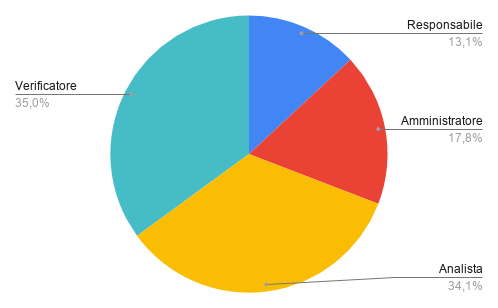
\includegraphics[width=12cm]{img/ruoli-analisi.png}
    \caption{Areogramma della suddivisione dei ruoli del periodo di Analisi}
    \label{fig:ore-ruolo-analisi}
  \end{figure}

\end{document}
